% =============================================================================
% COPYRIGHT AND DISCLAIMER
% =============================================================================
% This file is provided as a convenience template for competition participants.
% By using it, you accept full responsibility for compliance with all applicable
% copyright, licensing, and usage rules of the Association for Computing
% Machinery (ACM) and of any LaTeX packages you load (including, without
% limitation, the "acmart" document class and related ACM materials).
%
% Consult ACM's official publication, template, and copyright policies before
% using this setup for any purpose other than this competition. Do not assume
% that this template may be reused, redistributed, or submitted elsewhere
% without independently verifying ACM's current rules.
%
% Use of the "acmart" class, the "sigconf" option, or ACM-style formatting in
% this template does NOT mean that this report, this competition, its organizers,
% or any resulting PDF is sponsored, endorsed, affiliated with, or published by
% ACM. ACM trademarks and branding remain the property of ACM.
%
% Template packages live in preamble.tex.
% Citations live in main.bib. Edit this file with your paper content.
% =============================================================================


\documentclass[sigconf]{acmart}
% =============================================================================
% Template setup — participants normally do not edit this file.
% Author content belongs in main.tex; citations belong in main.bib.
% \documentclass lives in main.tex so Overleaf does not treat this file as root.
% =============================================================================

% --- Competition / non-ACM-submission friendly rights metadata -------------
\setcopyright{none}
\settopmatter{printacmref=false}
\acmConference[Kaggle Competition]{Filament Segmentation Challenge}{2026}{\href{https://www.kaggle.com/competitions/filament-segmentation-2026}{kaggle.com/competitions/filament-segmentation-2026}}
\acmBooktitle{Competition Report}
\acmDOI{}
\acmISBN{}

% --- Author guidance text --------------------------------------------------
% \guide{...} is gray italic while \guideStyletrue; omitted from the PDF if false.
% Flip the switch in main.tex after % =============================================================================
% Template setup — participants normally do not edit this file.
% Author content belongs in main.tex; citations belong in main.bib.
% \documentclass lives in main.tex so Overleaf does not treat this file as root.
% =============================================================================

% --- Competition / non-ACM-submission friendly rights metadata -------------
\setcopyright{none}
\settopmatter{printacmref=false}
\acmConference[Kaggle Competition]{Filament Segmentation Challenge}{2026}{\href{https://www.kaggle.com/competitions/filament-segmentation-2026}{kaggle.com/competitions/filament-segmentation-2026}}
\acmBooktitle{Competition Report}
\acmDOI{}
\acmISBN{}

% --- Author guidance text --------------------------------------------------
% \guide{...} is gray italic while \guideStyletrue; omitted from the PDF if false.
% Flip the switch in main.tex after % =============================================================================
% Template setup — participants normally do not edit this file.
% Author content belongs in main.tex; citations belong in main.bib.
% \documentclass lives in main.tex so Overleaf does not treat this file as root.
% =============================================================================

% --- Competition / non-ACM-submission friendly rights metadata -------------
\setcopyright{none}
\settopmatter{printacmref=false}
\acmConference[Kaggle Competition]{Filament Segmentation Challenge}{2026}{\href{https://www.kaggle.com/competitions/filament-segmentation-2026}{kaggle.com/competitions/filament-segmentation-2026}}
\acmBooktitle{Competition Report}
\acmDOI{}
\acmISBN{}

% --- Author guidance text --------------------------------------------------
% \guide{...} is gray italic while \guideStyletrue; omitted from the PDF if false.
% Flip the switch in main.tex after \input{preamble}.
%
% Do not use \guide{...} for \email{...}.
\usepackage{xcolor}
\newif\ifguideStyle
\guideStyletrue
\newcommand{\guide}[1]{%
  \ifguideStyle
    {\color{gray!65}\itshape #1}%
  \fi
}

% --- Math ------------------------------------------------------------------
% Do NOT load amssymb (or amsfonts): acmart already loads newtxmath, which
% defines the same symbols (e.g. \Bbbk) and causes a conflict on Overleaf.
% amsmath is already provided by acmart; mathtools extends it.
\usepackage{mathtools}

% --- Figures ---------------------------------------------------------------
% graphicx is already loaded by acmart
\usepackage{subcaption}

% --- Tables ----------------------------------------------------------------
% booktabs is already loaded by acmart
\usepackage{tabularx}
\usepackage{multirow}

% --- Bibliography style is set in main.tex (ACM-Reference-Format) ----------
.
%
% Do not use \guide{...} for \email{...}.
\usepackage{xcolor}
\newif\ifguideStyle
\guideStyletrue
\newcommand{\guide}[1]{%
  \ifguideStyle
    {\color{gray!65}\itshape #1}%
  \fi
}

% --- Math ------------------------------------------------------------------
% Do NOT load amssymb (or amsfonts): acmart already loads newtxmath, which
% defines the same symbols (e.g. \Bbbk) and causes a conflict on Overleaf.
% amsmath is already provided by acmart; mathtools extends it.
\usepackage{mathtools}

% --- Figures ---------------------------------------------------------------
% graphicx is already loaded by acmart
\usepackage{subcaption}

% --- Tables ----------------------------------------------------------------
% booktabs is already loaded by acmart
\usepackage{tabularx}
\usepackage{multirow}

% --- Bibliography style is set in main.tex (ACM-Reference-Format) ----------
.
%
% Do not use \guide{...} for \email{...}.
\usepackage{xcolor}
\newif\ifguideStyle
\guideStyletrue
\newcommand{\guide}[1]{%
  \ifguideStyle
    {\color{gray!65}\itshape #1}%
  \fi
}

% --- Math ------------------------------------------------------------------
% Do NOT load amssymb (or amsfonts): acmart already loads newtxmath, which
% defines the same symbols (e.g. \Bbbk) and causes a conflict on Overleaf.
% amsmath is already provided by acmart; mathtools extends it.
\usepackage{mathtools}

% --- Figures ---------------------------------------------------------------
% graphicx is already loaded by acmart
\usepackage{subcaption}

% --- Tables ----------------------------------------------------------------
% booktabs is already loaded by acmart
\usepackage{tabularx}
\usepackage{multirow}

% --- Bibliography style is set in main.tex (ACM-Reference-Format) ----------

\guideStylefalse
\setlength{\emergencystretch}{1em}
\begin{document}
\title{Family-Balanced Consensus with Bounded Contour Updates}
\subtitle{A Solution to the Solar Filament Segmentation Challenge 2026}
\author{Zhixiang Yang}
\affiliation{\country{China}}
\email{939295286@qq.com}
\begin{abstract}
This report describes our solution to the Solar Filament Segmentation Challenge 2026, a Kaggle competition on automatic segmentation of solar filaments in GONG H-$\alpha$ observations. We combine saved public predictions through five model-family votes, then improve contour agreement subject to explicit instance, topology and occupancy safeguards. Correlated models share a family weight. A conservative recall stage adds 13 corroborated instances, and a final SOLFIRE within-family update changes 359 contours without changing instance identities. The final 180-image, 1212-row file received a displayed public score of 0.41. Our contribution is prediction fusion and postprocessing; the component networks belong to their credited authors. The companion package verifies exact fusion replay by SHA256. Full upstream model-weight reconstruction remains incomplete and is explicitly disclosed; no claim of complete end-to-end final-judging reproducibility is made.
\end{abstract}
\maketitle
\section{Introduction}
This report goes over the details of our submitted solution to the Solar Filament Segmentation Challenge~2026 \cite{filament-segmentation-2026}. The challenge, launched on July~10,~2026, is organized by the Earth-Space AI Research (ESAIR) Lab\footnote{\href{https://www.esairlab.com/home}{www.esairlab.com/}}. This challenge utilizes the MAGFiLO dataset for evaluation of the segmentation algorithms \cite{ahmadzadeh2024dataset}.

Our starting point is an attributed public five-family existence vote by prvsiyan~\cite{prvsiyan2026}. This vote establishes which instances survive but inherits mask geometry from source traversal and overlap removal. We retain its instance identities and replace eligible contours by a family-balanced majority. The design seeks a bounded change with a transparent audit trail, rather than estimating accuracy from prediction agreement.

The final method performs no gradient updates and uses no hidden test labels. It consumes compressed RLE prediction files at native $2048\times2048$ resolution. Its inputs were produced by public segmentation systems, including UNet-based networks, direct and crop-based YOLO variants, and Mask R-CNN. We do not claim these architectures or their training as our own. Source versions and file hashes are pinned to prevent silently changing an experiment when a public notebook is updated.

\section{Methodology}
\subsection{Inputs, families and provenance}
The original voter set comprises seven files: two Tush predictions and one historical Dariush prediction in the UNet family; one HDJoJo direct-YOLO prediction; the MAGFiLO crop-YOLO26 prediction; the Tim crop-YOLO11 prediction; and a Mask R-CNN threshold-0.70 intermediate. We subsequently replace the direct source by HDJoJo V2, which combines YOLO26x and YOLOv8x. Those two models still receive only one family vote. The final SOLFIRE source~\cite{solfire2026} is averaged inside the existing UNet family, not counted as an independent sixth family.

\begin{table}[h]
\caption{Pinned public prediction sources. Versions identify saved artifacts, not retrained models. Complete byte hashes and credits are in the companion package.}
\label{tab:inputs}
\small
\begin{tabular}{lll}\toprule
Family & Contributor / source & Version \\\midrule
UNet & Tush, two sources & 354107337 / 351734356\\
UNet & Dariush, historical V2 & 359486068\\
UNet & SOLFIRE, final update & 369652646\\
Direct YOLO & HDJoJo, historical / latest & 367892109 / 369397665\\
Crop YOLO26 & Muhammad Shoaib Altaf & 362037449\\
Crop YOLO11 & Tim Gluhkikh & 342770268\\
Mask R-CNN & Public threshold intermediate & thr070\\\bottomrule
\end{tabular}
\end{table}

All files are decoded on the same pixel grid and grouped by image stem. An absent image in one source provides no support. No images or annotations are used to fit fusion parameters. The original 1199-row anchor is regenerated from the pinned voters; it is not substituted with an unrelated CSV or hidden output. Historical Dariush V2 is necessary because its newer output differs. Nine input CSVs suffice for the complete fusion replay, including the historical and updated direct sources.

\clearpage
\subsection{Existence voting and mask correspondence}
The public baseline retains an instance when at least three distinct families support it at intersection over union (IoU) strictly greater than 0.5; exactly three supporters require each best correspondence to reach 0.6. Original source-order selection, reservation of previously occupied pixels and fallback behavior are replayed without modification. This reproduces the 1199-row anchor exactly. The seed is the original public ensemble, not the separately developed single-fold ConvNeXt system.

For contour updates, correspondence is more restrictive: a source mask and an anchor must be mutual best IoU matches, with IoU above 0.5. The three-family condition and its 0.6 restriction remain. SOLFIRE additionally requires a mutual anchor match at IoU at least 0.6. This avoids freely adding source pixels from weak correspondences. A source cannot supply multiple independent family votes simply because it contains several related checkpoints or networks.

\subsection{Family-balanced geometry}
Let $A_i$ be the original anchor, $M_{ifj}$ a matched source mask in family $f$, and $n_{if}$ the number of matched masks within that family. Each family contributes
\begin{equation}
v_{if}(x)=\frac{1}{n_{if}}\sum_{j=1}^{n_{if}}\mathbb{1}[x\in M_{ifj}],\qquad
V_i(x)=\sum_{f\in F_i}v_{if}(x).
\end{equation}
The proposal contains pixels with $V_i(x)>|F_i|/2$. Exact ties preserve the anchor pixel. The computation includes anchor and source union pixels; pixels already reserved by other retained instances are removed before evaluation. Thus an ensemble with three correlated UNet files does not outweigh three different families by raw model count.

An update must meet all of the following guards: IoU to the protected mask at least 0.8; area ratio between 0.8 and 1.25; unchanged number of eight-connected components; a strict increase in the equal-family mean of source IoUs; and no decrease in the count of families whose mean source IoU exceeds 0.5. If simultaneous expansions conflict, every conflicting update reverts. We do not settle collisions by an arbitrary source order.

The final within-family SOLFIRE stage applies the geometry and topology guards to both the current mask and the original anchor. Computing from the anchor limits cumulative contour drift. The 13 masks added by the earlier recall stage are preserved exactly. Of the 1212 final rows, 359 contours on 148 images change relative to that preceding 1212-row control. Minimum accepted IoU is 0.804205 to current and 0.801233 to anchor. These are safety diagnostics; they do not measure segmentation accuracy.

\begin{figure}[h]
\centering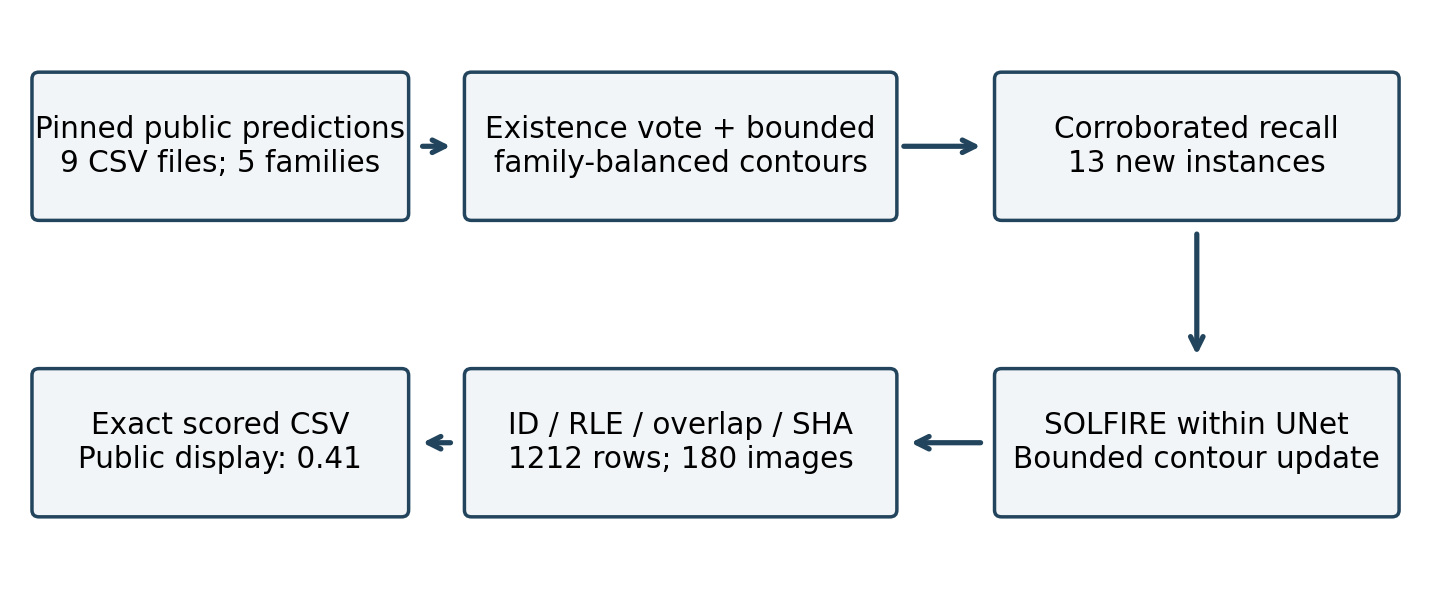
\includegraphics[width=\linewidth]{pipeline.png}
\caption{The executable prediction-fusion pipeline. The upstream image-to-network inference stage is external and is not reconstructed by this package. All five generated CSV stages are checked against frozen hashes.}
\label{fig:pipeline}
\end{figure}

\subsection{Conservative recall supplement}
Before the final contour update, HDJoJo V2 detections missing from the anchor may enter a separate recall stage. A candidate has maximum IoU 0.5 to the retained set and at most 10\% foreground overlap. It needs mutual-best support at IoU at least 0.6 from three distinct families including direct YOLO. Its family-balanced majority must retain IoU at least 0.8 to the direct candidate, the same area interval and component count. After removing occupied pixels, at least 90\% of its pixels and three supporting family matches at IoU at least 0.6 must remain. Conflicting additions are rejected together. Thirteen instances on thirteen images pass, taking the row count from 1199 to 1212; their final areas range from 281 to 3326 pixels.

\clearpage
\section{Evaluation}
\subsection{Public results and selection}
The final artifact has already received a successful Kaggle scoring receipt. The displayed public score is 0.41. The last directly verified leaderboard position was 147 of 1548 teams (approximately the top 9.50\%) on November 15, 2026, with 15 cumulative submissions. This is a dated public observation, not the final private result. The chosen file is the first entry on the observed Public Score-sorted submission list. Several entries display 0.41; the platform's limited decimal display cannot establish exact equality of their hidden-precision scores.

\begin{table}[h]
\caption{Observed public submission results. All rows use real scoring receipts. ``0.41'' denotes the displayed value, not an independently measured unrounded score.}
\label{tab:results}
\small
\begin{tabular}{lrr}\toprule
Submitted method & Rows & Public display\\\midrule
Earlier in-house cascade / ConvNeXt control & 1192 & 0.39\\
Attributed five-family baseline replay & 1199 & 0.40\\
Family-balanced contour consensus & 1199 & 0.41\\
Updated direct source + contour consensus & 1199 & 0.41\\
Corroborated direct recall supplement & 1212 & 0.41\\
SOLFIRE within-family boundary (final) & 1212 & 0.41\\\bottomrule
\end{tabular}
\end{table}

Family-balanced contour consensus produced the first demonstrated displayed improvement from 0.40 to 0.41. Later direct-source replacement and the recall stage coincided with observed public rank advances, but no unrounded score was available. The final SOLFIRE contour stage produced no demonstrated displayed score or rank improvement relative to the preceding control. We retain that control and all fingerprints rather than describing every contour change as a gain. A separate SOLFIRE recall experiment added another 13 masks, yielded no demonstrated gain and is not included in this final file.

The original public test metric is evaluated by the host on an approximately half-test public subset. We do not possess those labels, per-image public scores or private scores. Confidence intervals for the final public ensemble therefore cannot be calculated from the available evidence. Repeated public submissions also introduce model-selection bias. Agreement-based diagnostics on the test predictions are explicitly not held-out PQ or evidence of true positives.

\subsection{Separate labelled development evidence}
Earlier work evaluated a trainable ConvNeXt quality refiner on a single-fold cascade OOF set. This evidence belongs to the earlier 0.39 pipeline and is not a matched validation set for the final public ensemble. It used 48 calibration images and 129 repeatedly examined development images. Training excluded these 177 images; the pilot saw 143 of 530 training images, 3380 crops, 6327 optimizer updates, and selected epoch 12 at 5076 updates. On the 129-image development set, PQ changed from 0.45275035 to 0.46325567, paired difference 0.01050532, with a paired 95\% bootstrap interval [0.0021516, 0.0193779] and 24 additional true positives. The corresponding test submission still displayed 0.39. This demonstrates why development improvements cannot be equated with leaderboard improvement.

A later zero-training SAM 2.1 prompt-refinement diagnostic also failed on the same frozen development predictions. Raw refinement gave PQ 0.31735074 versus the 0.45275035 control, difference $-0.13539961$. Its paired 95\% interval ran from $-0.15427336$ to $-0.11771649$. Guarded refinement gave PQ 0.39249304, difference $-0.06025731$, with an interval from $-0.07044308$ to $-0.05057692$. Neither became a test submission. These intervals describe this development diagnostic alone; they do not transfer to the 0.41 ensemble. No rejected architecture is represented as a successful part of the final solution.

\subsection{Artifact validation}
The exact final CSV is checked for column names, unique sequential instance IDs, all 180 image stems, canonical COCO compressed RLE, decoded dimensions, legal empty images, pairwise pixel disjointness and CSV readback. Byte identity is enforced by SHA256. Every generated intermediate is also hash-checked, so a threshold change or different historical input cannot silently be called the submitted method. Output validation establishes format and deterministic replay, not scientific correctness or final eligibility.

\clearpage
\subsection{Qualitative mask changes}
Figure~\ref{fig:masks} shows six deterministic, area-stratified examples from the final contour changes. The panels display binary masks on a neutral background, not a solar-image overlay or annotation comparison. Shared pixels are dark gray; pixels removed from the preceding control are orange and added pixels are cyan. The examples illustrate bounded changes in thin structures and irregular edges. They cannot establish whether those changes follow the correct annotator interpretation.

\begin{figure}[h]
\centering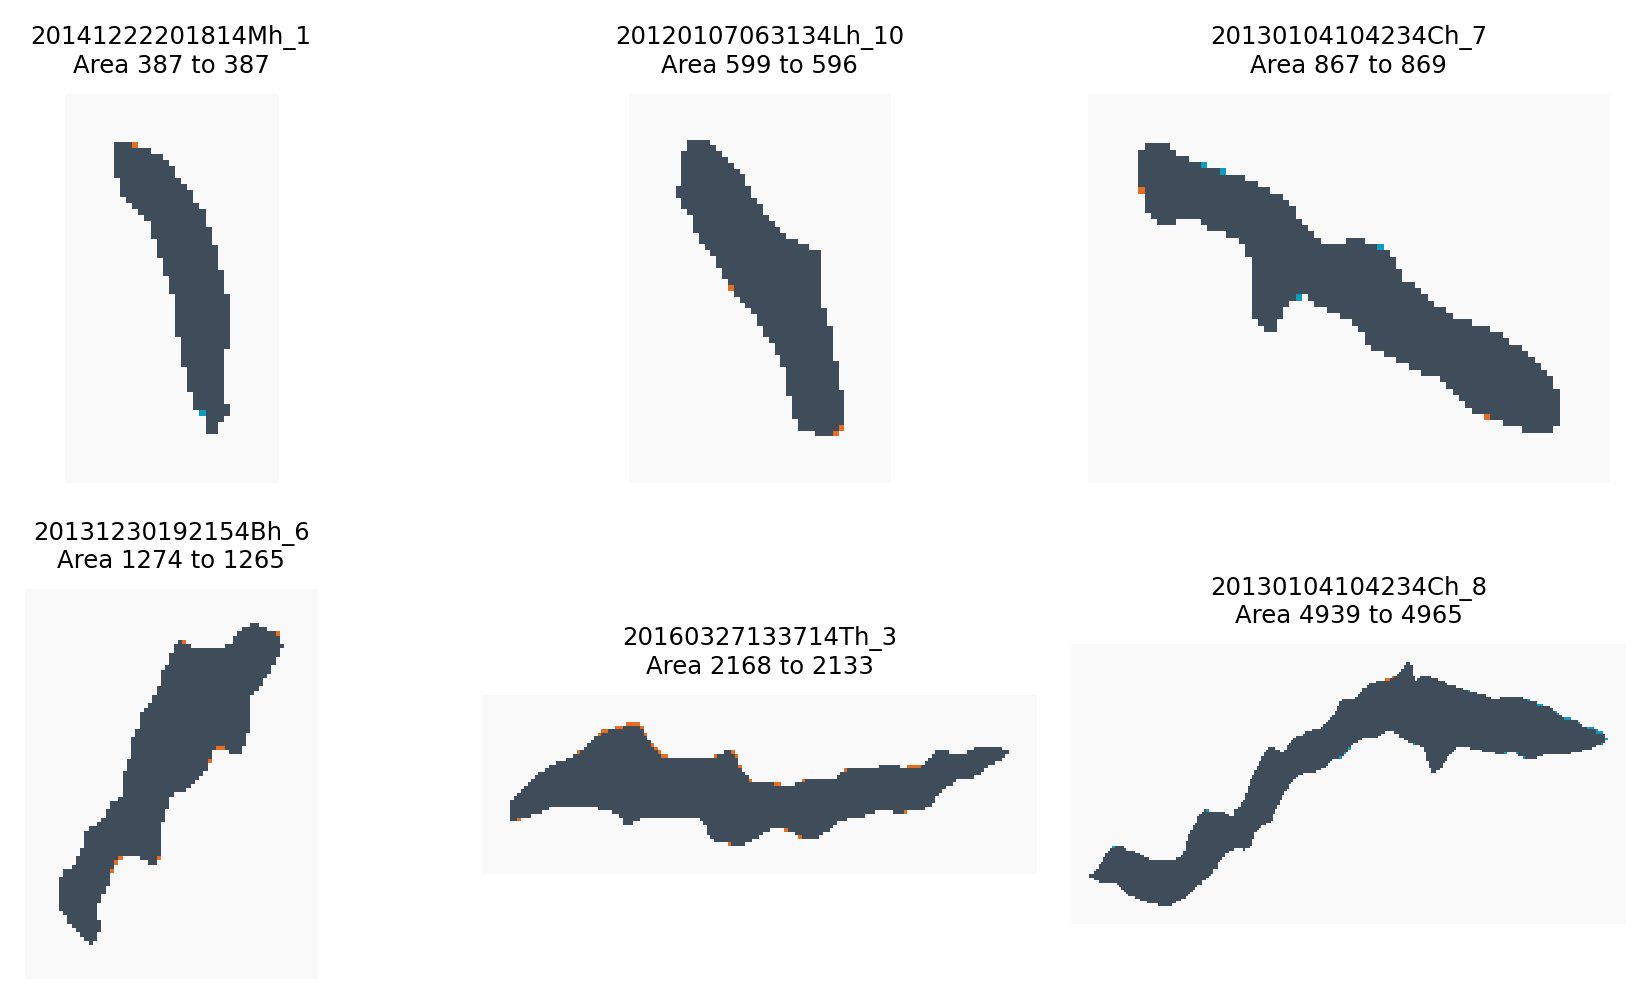
\includegraphics[width=\linewidth]{mask_examples.png}
\caption{Mask-only examples from the final SOLFIRE within-family update, selected at the 5th, 20th, 40th, 60th, 80th and 95th area percentiles of changed instances. Native-pixel crops are independently scaled for visibility. Gray: retained in both; orange: removed; cyan: added. No ground truth is shown.}
\label{fig:masks}
\end{figure}

\section{Reproducibility, scope and limitations}
\subsection{What the package reproduces}
The companion package includes nine pinned public prediction CSVs, the 180 image IDs, the original voting-function excerpt, all fusion modules and protocol files, a Jupyter notebook, a CLI, exact dependency versions, attribution and SHA256 manifests. It regenerates the baseline and each subsequent stage in a new output directory. The final file is not used as an input to manufacture an apparent replay. The required final fingerprint is
\begin{center}\small\ttfamily
68b26327bd9770d621753144ec29220af0\\
e2b40094ee5756953af41409c94a09
\end{center}
with no newline between the two displayed segments. The actual file uploaded with this report must be byte-identical to that already scored CSV. The environment tested for fusion uses Python 3.13.5, NumPy 2.1.3, pandas 2.2.3, SciPy 1.15.3 and pycocotools 2.0.11. Portability edits remove a workstation-specific dependency path and replace a previously saved seed's image-list lookup with an explicit image-ID file. The mask algorithms and thresholds remain unchanged.

\subsection{End-to-end reconstruction gap}
The package reproduces postprocessing from saved public predictions. It does not supply every exact upstream network weight, verified training split or complete image-to-network dependency environment for all five families. We have not independently reconstructed those networks from original images. Accordingly, this package does not establish that the competition's full public model-code-and-weight reproducibility requirement is satisfied. We disclose this limitation for the organizing committee's eligibility decision; the successful public scoring receipt alone cannot resolve it. We do not relabel public predictions as independently trained weights or claim third-party architectures as novel contributions.

The conservative guards also impose a scientific limitation: preserving the anchor's instance set and component count can preserve incorrect splits, merges and missed objects. Family errors are correlated even across the five coarse groups. Requiring three families may suppress valid small structures observed by fewer systems. Strict mask agreement may favor shared errors, and the limited public subset can reward a rule that does not generalize to the private subset. Stronger future work would build matched labelled OOF predictions for every source, test instance-existence and topology rules there, and provide all upstream inference code and frozen weights. This has not been completed for the submitted ensemble.

\subsection{Attribution and AI assistance}
Public prediction contributors include Tush, Dariush Afshar, HDJoJo, Muhammad Shoaib Altaf, Tim Gluhkikh, Fususu / phuongncn, Nomannic19, prvsiyan and Vedran Hrabar. Their source/version ledger accompanies the code. Apache-2.0 was observed for the prvsiyan and SOLFIRE notebooks; no blanket license or redistribution right is asserted for every underlying third-party artifact. AI assistance supported implementation, debugging, analysis and report drafting. No hidden labels, fabricated measurements or AI-generated benchmark scores were used. The description distinguishes original contributions, source-derived components, measured results and unresolved reproducibility requirements.

\clearpage
\section{Acknowledgment}\label{sec:acknowledgment}
    % Do not change
    The organization of the Filament Segmentation Challenge 2026 is partially supported by the U.S. National Science Foundation (NSF) under Grant No. 2209912 and 2433781, directorate for Computer and Information Science and Engineering (CSE), and Office of Advanced Cyberinfrastructure (OAC), and Grant No. 2511630, AST Division Of Astronomical Sciences and MPS Directorate for Mathematical and Physical Sciences.

    The Filament Segmentation Challenge 2026 is sponsored by the U.S. National Science Foundation (NSF) National Solar Observatory (NSO). 

    This work utilizes GONG data obtained by the NSO Integrated Synoptic Program, managed by the National Solar Observatory, which is operated by the Association of Universities for Research in Astronomy (AURA), Inc. under a cooperative agreement with the National Science Foundation and with contribution from the National Oceanic and Atmospheric Administration. The GONG network of instruments is hosted by the Big Bear Solar Observatory, High Altitude Observatory, Learmonth Solar Observatory, Udaipur Solar Observatory, Instituto de Astrofísica de Canarias, and Cerro Tololo Interamerican Observatory.


\bibliographystyle{ACM-Reference-Format}
\bibliography{main}
\end{document}
